Based on the experience of previous project, the team chose the spiral model
of software development methodologies. A spiral model is a form of 
risk-driven development where the most risky parts of a project are 
identified early and planned into prototypes that can inform the final 
product. See the breakdown of the prototypes the team chose in table \ref{sec:progress:prototypes-table}.

\begin{table*}[!htbp]
\caption{Prototypes and Schedules}
\label{sec:progress:prototypes-table}
\begin{center}
\begin{tabular}{  l  l p{10cm} }
	\bf Schedules & \bf Prototypes/Work & \bf Descriptions\\ \hline \\
	Week 1 & Planning and Pre-survey & Get the original project to work, plan a few changes and enhacenments, do a user survey\\
	Week 2 & Project Proposal & Detail the plan and get ready the project proposal\\
	Week 3-1 & Prototype 1 & Gernerate dummy data, build loading history interface\\
	Week 3-2 & Prototype 2 & Gernerate dummy data, build suggestion interface\\
	Week 4-1 & Prototype 3 & Build suggestion algorithm and intergated into final system \\
	Week 4-2 & Prototype 4 & System evaluation, user testing, update system \\
	Week 5 & Presentation & Present the final system \\
	Week 6/7 & Final Paper & Draft and finalize the paper \\
\end{tabular}
\end{center}
\end{table*}


This afforded the team the ability to have regular check-ins and to measure
progress against the prototypes. The team will convene two to three times 
a week to do pair programming and to check progress against the prototypes.
When combined with regular check-ins with the TAs, the team shall be able 
to build prototype programs to perform design feature and functionality.

We also used Gitup project boards to create and track our progress. This 
method featured the ability to send a notification to the team member to 
remind and collaborate within the team members. Here is the example image.

\begin{table}[ht]
\caption{Progress Tracking Board}
\label{section:progress:tracking-board}
\centering
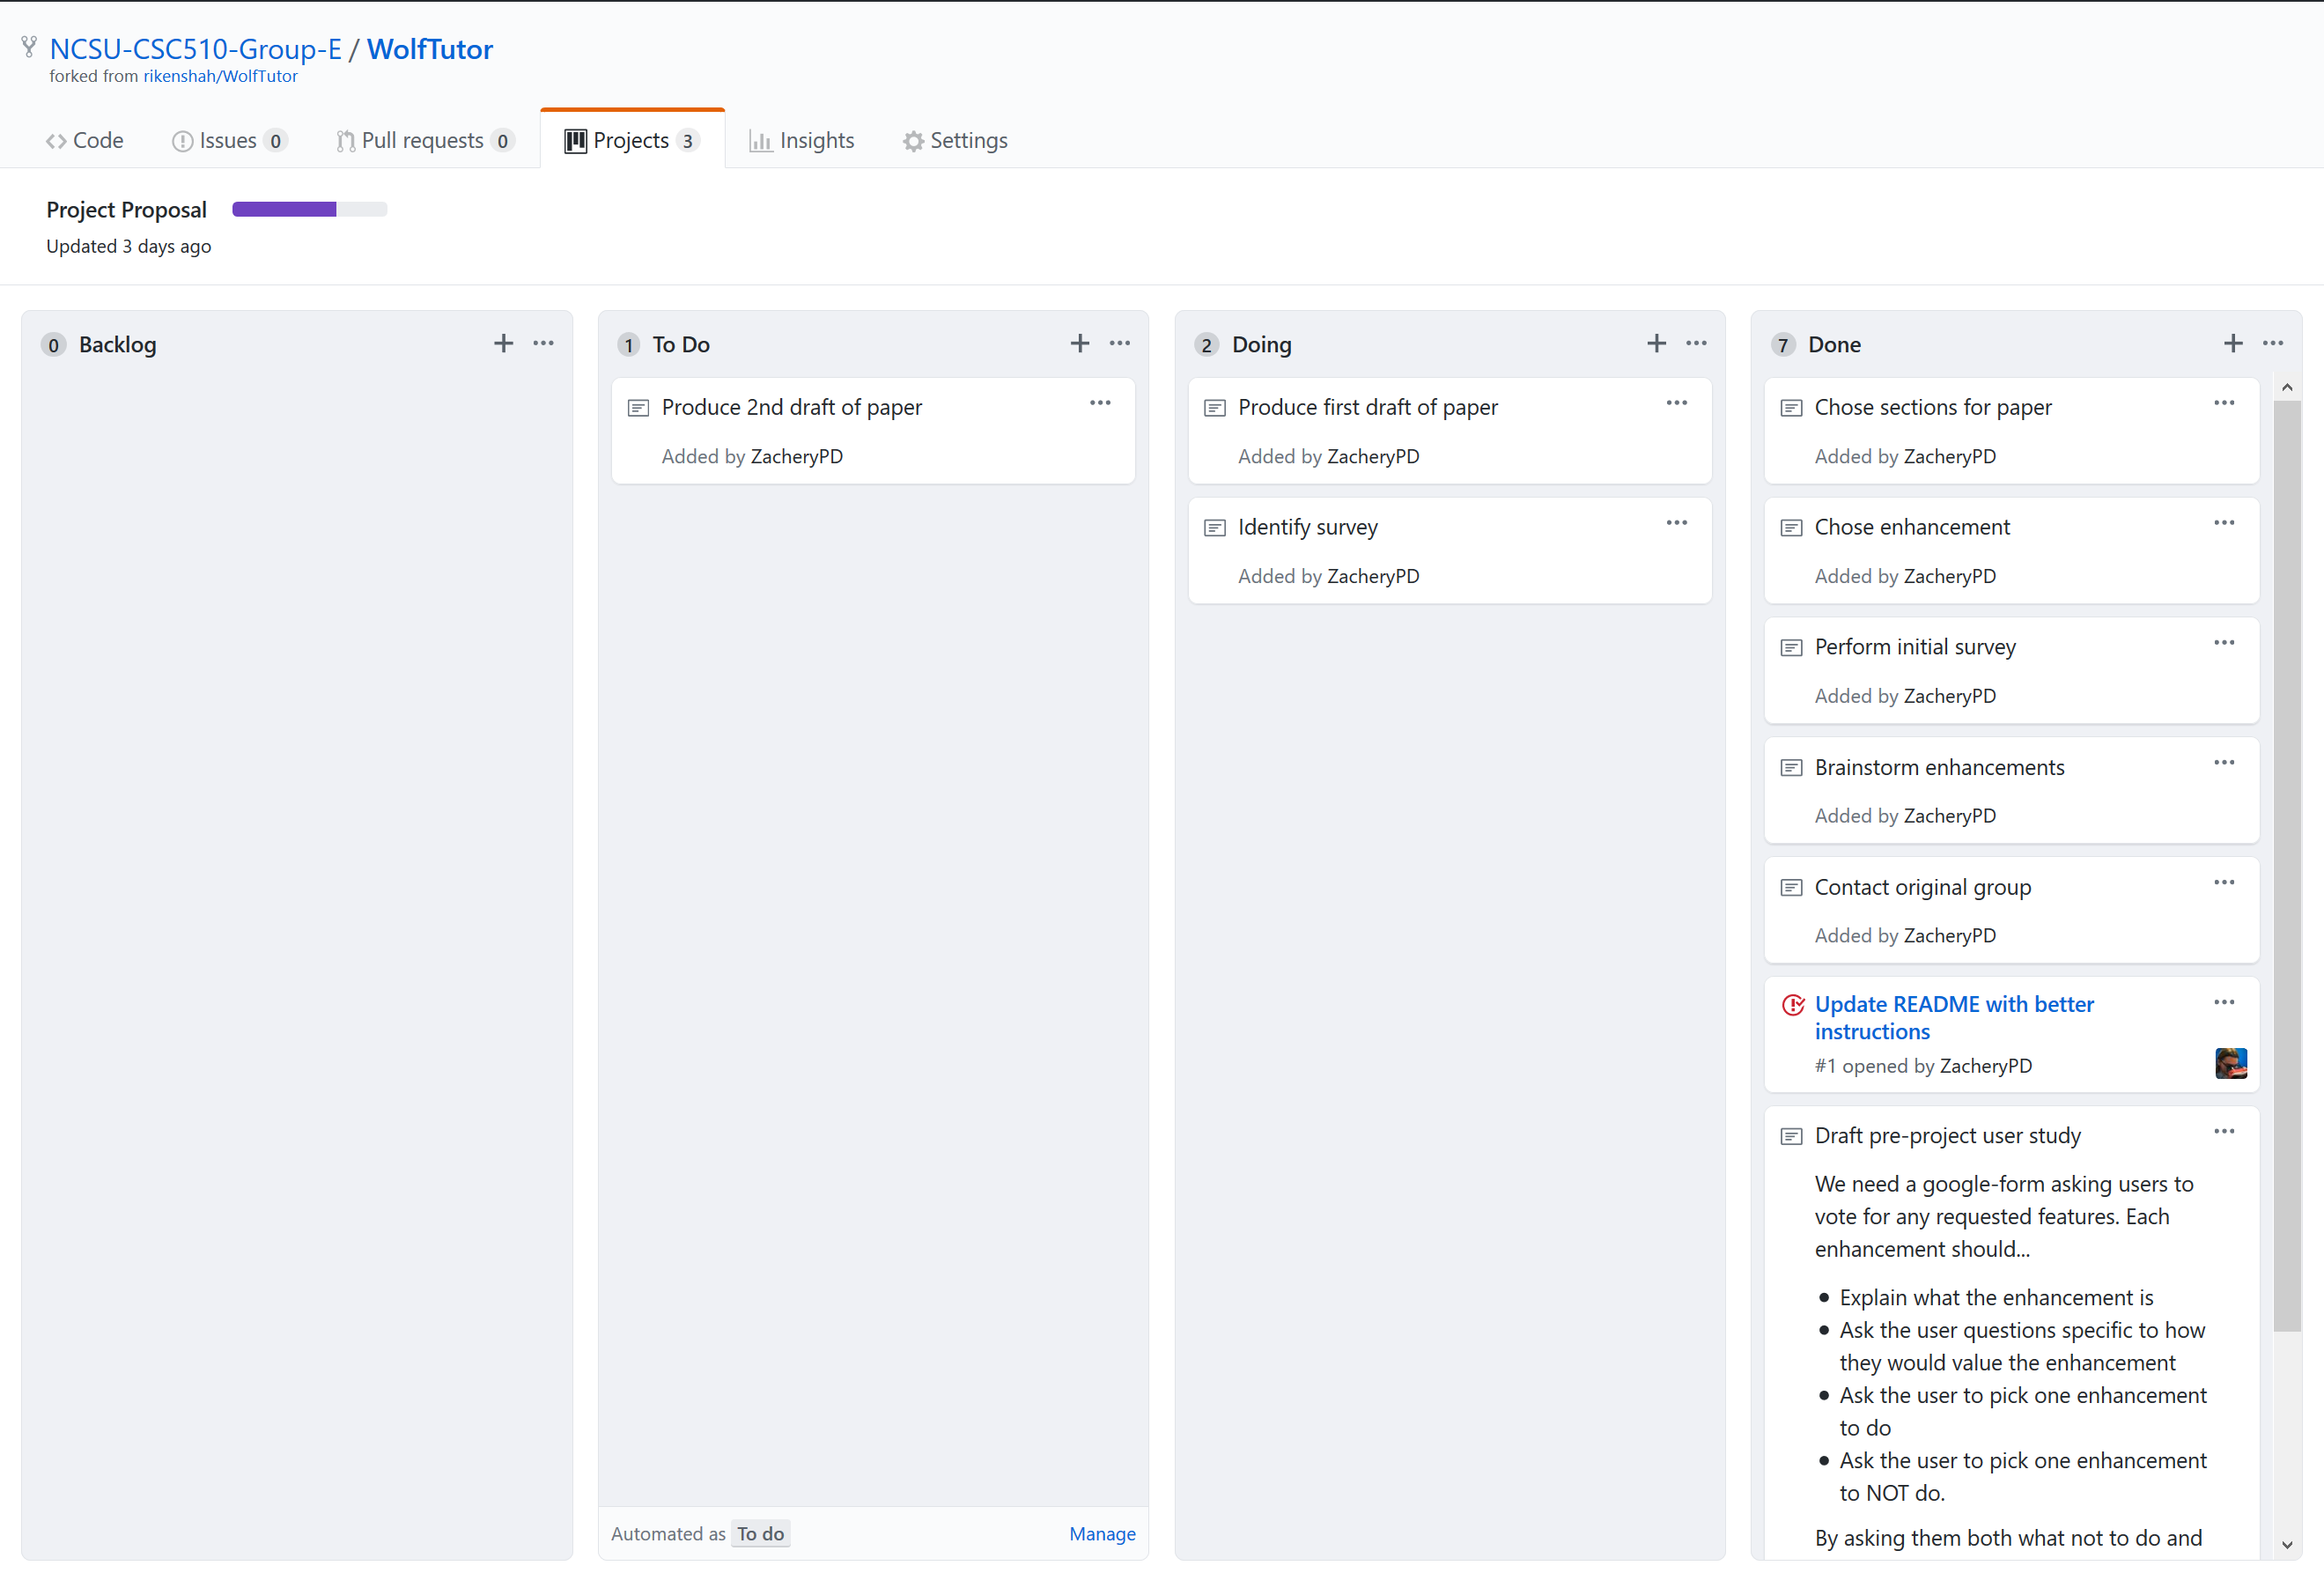
\includegraphics[width=0.48\textwidth]{progress.png}
\end{table}